\documentclass[12pt, twoside]{article}
\usepackage[letterpaper, margin=1in, headsep=0.5in]{geometry}
\usepackage[english]{babel}
\usepackage[utf8]{inputenc}
\usepackage{amsmath}
\usepackage{amsfonts}
\usepackage{amssymb}
\usepackage{tikz}
%\usetikzlibrary{quotes, angles}

\usepackage{graphicx}
\usepackage{enumitem}
\usepackage{multicol}

\usepackage{fancyhdr}
\pagestyle{fancy}
\fancyhf{}
\renewcommand{\headrulewidth}{0pt} % disable the underline of the header

\fancyhead[RE]{\thepage}
\fancyhead[RO]{\thepage \\ Name: \hspace{3cm}}
\fancyhead[L]{BECA / Dr. Huson / 12.1 IB Math SL\\* 22 January 2019}

\begin{document}
\subsubsection*{Spiral Review: 1-1 P1 (No Calculator) Algebra Sequences}
 \begin{enumerate}

  \item 17M.1.sl.TZ2.1
  \begin{enumerate}
    \item In an arithmetic sequence, the first term is 3 and the second term is 7.\\
    Find the common difference. [2 marks]
    \item Find the tenth term. [2 marks]
    \item Find the sum of the first ten terms of the sequence. [2 marks]
  \end{enumerate}

  \item 17N.1.sl.TZ0.2
  \begin{enumerate}
    \item In an arithmetic sequence, the first term is 8 and the second term is 5.\\
    Find the common difference. [2 marks]
    \item Find the tenth term. [2 marks]
    \item Find the sum of the first ten terms. [2 marks]
  \end{enumerate}

  \item 14N.1.sl.TZ0.2
  \begin{enumerate}
    \item In an arithmetic sequence, the first term is 2 and the second term is 5.\\
    Find the common difference. [2 marks]
    \item Find the eighth term. [2 marks]
    \item Find the sum of the first eight terms of the sequence. [2 marks]
  \end{enumerate}

  \item 14M.1.sl.TZ1.2
  \begin{enumerate}
    \item In an arithmetic sequence, the third term is 10 and the fifth term is 16.\\
    Find the common difference. [2 marks]
    \item Find the first term. [2 marks]
    \item Find the sum of the first 20 terms of the sequence. [3 marks]
  \end{enumerate}

  \item 11M.1.sl.TZ2.1
  \begin{enumerate}
    \item In an arithmetic sequence, $u_1=2$ and $u_3=8$.\\
    Find $d$. [2 marks]
    \item Find $u_{20}$. [2 marks]
    \item Find $S_{20}$. [2 marks]
  \end{enumerate}

  \item Three consecutive terms of a geometric sequence are $x-3$, $6$ and $x+2$.\\
  Find the possible values of $x$.\\
  16M.1.sl.TZ2.4  [6 marks]

  \item 08N.1.sl.TZ0.1
  \begin{enumerate}
    \item Consider the infinite geometric sequence $3, 3(0.9), 3(0.9)^2, 3(0.9)^3,\dots$.\\
    Write down the 10th term of the sequence. Do not simplify your answer. [1 mark]
    \item Find the sum of the infinite sequence. [4 marks]
  \end{enumerate}

  \item 10N.1.sl.TZ0.1
  \begin{enumerate}
    \item The first three terms of an infinite geometric sequence are 32, 16 and 8.\\
    Write down the value of r. [2 marks]
    \item Find $u_6$. [2 marks]
    \item Find the sum to infinity of this sequence. [2 marks]
  \end{enumerate}

  \item 16M.1.sl.TZ1.4
  \begin{enumerate}
    \item Consider the following sequence of figures.
    \begin{center}
      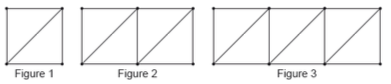
\includegraphics[width=0.6\textwidth]{1-1-P1_Algebra-8.png}
    \end{center}
    Figure 1 contains 5 line segments.\\
    Given that Figure $n$ contains 801 line segments, show that $n=200$.[3 marks]
    \item Find the total number of line segments in the first 200 figures. [3 marks]
  \end{enumerate}

  \item 16M.1.sl.TZ1.4
  \begin{enumerate}
    \item Consider the arithmetic sequence $2, 5, 8, 11, \dots$.\\
    Find $u_{101}$.[3 marks]
    \item Find the value of $n$ so that $u_n = 152$. [3 marks]
  \end{enumerate}

  \item 15N.1.sl.TZ0.7 \\
    An arithmetic sequence has the first term $\ln a$ and a common difference $\ln 3$.\\
    The 13th term in the sequence is $8 \ln 9$. Find the value of $a$. [6 marks]


  \item 18M.1.sl.TZ2.7
  \begin{enumerate}
    \item An arithmetic sequence has $u_1 = \log_c(p)$ and $u_2 = \log_c(pq)$, where $c>1$ and $p, q>0$.\\
    Show that $d = \log_c(q)$. [2 marks]
    \item Let $p=c^2$ and $q=c^3$. Find the value of $\displaystyle \sum_{n=1}^{20} u_n$. [6 marks]
  \end{enumerate}

  \item 17M.1.sl.TZ1.7
  \begin{enumerate}
    \item The first three terms of a geometric sequence are $\ln x^{16}, \ln x^8, \ln x^4$, for $x>0$.\\
    Find the common ratio. [3 marks]
    \item Solve $\displaystyle \sum_{k=1}^{\inf} 2^{5-k} \ln x = 64$. [5 marks]
  \end{enumerate}


\item 17N.1.sl.TZ0.10a
\begin{enumerate}
  \item The following diagram shows [AB], with length 2 cm. The line is divided into an infinite number of line segments. The diagram shows the first three segments.
  \begin{center}
    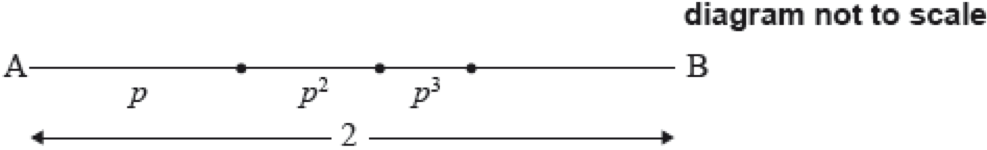
\includegraphics[width=0.6\textwidth]{1-1-P1_Algebra-14a.png}
  \end{center}
  The length of the line segments are $p$ cm, $p^2$ cm, $p^3$ cm, ..., where $0<p<1$.\\
  Show that $p=\frac{2}{3}$.[5 marks]
  \item The following diagram shows [CD], with length $b$ cm, where $b>1$. Squares with side lengths $k$ cm, $k^2$ cm, $k^3$ cm, ..., where $0<k<1$. are drawn along [CD]. This process is carried on indefinitely. The diagram shows the first three squares.
  \begin{center}
    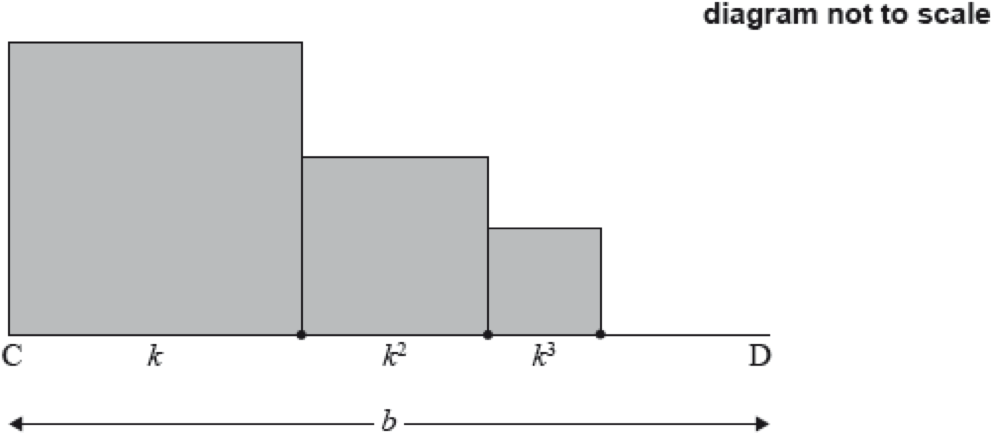
\includegraphics[width=0.6\textwidth]{1-1-P1_Algebra-14b.png}
  \end{center}
  The \emph{total} sum of the areas of all of the squares is $\frac{9}{16}$. Find the value of $b$. [9 marks]
\end{enumerate}

\item 18M.1.sl.TZ1.10
\begin{enumerate}
  \item The first two terms of an infinite geometric sequence are $u_1 =18$ and $u_2=12 \sin^2 \theta$, where $0< \theta < 2\pi$.\\
  Find an expression for $r$ in terms of $\theta$. [2 marks]
  \item Find the possible values of $r$. [3 marks]
  \item Show that the sum of the infinite sequence is $\frac{54}{2+ \cos (2\theta)}$. [4 marks]
  \item Find the values of $\theta$ which give the greatest value of the sum. [6 marks]
\end{enumerate}


  \newpage




\end{enumerate}
\end{document}
